%!TEX root = ../BoYu-Dissertation.tex
\graphicspath{{Figures/}}

\chapter{Our Approach: Overview} % (fold)
\label{cha:our_approach_overview}

Our approach to supporting awareness in complex, distributed geo-collaborative activities aims to address the two major design challenges identified in Section \ref{sec:review_discussion}: 

\begin{enumerate}
   \item As neither space-based nor event-based models in existing studies can effectively support awareness processes in collaborative activities when both the complexity and dynamics scale up, a new awareness model that can leverage the strengths of both space-based and event-based models becomes extremely important.
   \item By conceptualizing the awareness phenomena in complex, distributed collaborative activities as a continuous development of awareness knowledge through a variety of integrated cognitive and social processes, it is very important to consider the awareness support from a collective perspective and provide integrated support for the whole awareness development cycle.
\end{enumerate}

This chapter provides an overview of our approach. The general design principle of our approach is to emphasize the active role of computer system to not merely support, but rather promote awareness in complex collaborative activities. In the following, we first describe the design concept of awareness promotion, and then describe the major components of our awareness promotion framework.

\section{From Awareness Support to Awareness Promotion} % (fold)
\label{sec:from_support_to_promotion}
In order to address the design challenges of scaling up and integrated support, we argue that the computer system needs to play an active role to promote awareness among collaborators. Our awareness promotion approach has its basis in two basic parent disciplines:  artificial intelligence (AI) and human-computer interaction (HCI). 
\begin{enumerate}
   \item From AI, we consider the computer as \emph{an active agent} \cite{Brown99activeuser}, situated within the collaborative environment that adaptively sense, acts, and reacts within this environment over time, to pursue its goal of promoting awareness.
   \item From HCI, we act on the premise that computers and humans have fundamentally asymmetric abilities \cite{Dalal1994}; therefore, we focus on developing divisions of responsibility that exploit the strengths and overcome the weaknesses of both, and utilizing interaction techniques to facilitate effective \emph{human-computer collaboration} \cite{Terveen1995}.
\end{enumerate}

\subsection{The role of computer: from tool to actor} % (fold)
\label{sub:the_role_of_computer}
In existing awareness systems, the role of computer can be described in the metaphor of `tool'. The `tool' perspective emphasizes the human achieves his/her goal through the computer application \cite{Bodker1997}. In term of supporting awareness, it means the human actors use the computer to achieve awareness. The tool perspective emphasizes the control on the human user's side, and how the computer is used to achieve awareness depends on the human user's own knowledge. For example, in space-based systems, the system relies on the user to monitor the shared space to perceive awareness information; in event-based systems, the user needs to explicitly express his/her interests so that the computer can filter out events. 

However, when the collaborative activities become more and more distributed and complicated, more is demanded of the user to control the computer. As we conceptualize the awareness phenomena as a distributed cognitive system (Section \ref{sec:integrated_conceptual_model_of_awareness}), each user usually only have partial knowledge about the whole collaborative situation, and it is unlikely that the user will have the full knowledge of what exactly should be done in order to achieve awareness as a group. The user may have no idea what background information should be attended to in order to interpret a piece of awareness information that is out of his/her local scope of work. Or he/she cannot decide on who should be notified when his/her activities are changed. As a result, the user either uses the partial knowledge to develop awareness that is often incomplete, vague, or even incorrect; or has to extend the mental model to represent more knowledge that out of his/her local scope of work, which inevitably increases the user's cognitive load. 

As a result, we believe that merely relying on the user to control the computer as a `tool' to achieve awareness in distributed, complex collaboration is ineffective. Alternatively, a better approach is to allow the computer to take some control away from the user and actively perform some tasks to help the user to achieve awareness. Instead of relying on the user's internal, partial knowledge to control the awareness development, the computer can maintain a much more complete knowledge representation of the whole field of work at the systematic level, and make use of this knowledge to infer the user's need in the various awareness processes so as to provide awareness support. In this way, the computer can be considered as a `mediator' actively engaged in the collaborative activities along with human actors, but with its own goal (i.e. to assist human actors to achieve awareness), its own mental model (i.e. the knowledge representation of the whole field of work), and its own behaviors (i.e. the capabilities to reason about the user's need in the various awareness processes and adapt interaction and information presentation techniques to support it).
% subsection the_role_of_computer (end)

\subsection{Human computer collaboration} % (fold)
\label{sub:human_computer_collaboration}
While considering the computer as an active actor to support awareness, it does not mean we can delegate all the tasks to the computer and build a completely automatic system. Existing studies in HCI and cognitive science have suggested that the relationship between human users and artificial intelligence should be treated as joint cognitive systems \cite{Dalal1994} or human-computer collaboration systems \cite{Terveen1995}, emphasizing the appropriate partition of responsibility between human actors and computer systems. This perspective of human computer interaction is based on two premises.

\begin{enumerate}
   \item It begins with the premise that computers and humans have fundamentally asymmetric abilities. The computer's strength lies in its ability to store more information than can be stored in the human's short-term memory, to perform faster data retrieval and processing, and to conduct more reliable low-level routine inferences \cite{Brown99activeuser}. On the other hand, the human's strength lies in the ability to integrate information from multiple sources to provide insight necessary to draw complex, higher level inferences, and the capability to handle unexpected situations with the help of long-term memory, experiences, and even intuition. As a result, the goal of computer support is actually to investigate the relationship between the cognitive characteristics of the human and the cognitive characteristics of the computer, and get the computer to complement the human \cite{Dalal1994}.
   \item It assumes that the human and the computer be cooperative to each other in the interaction. It means not only the computer will keep track of the human's activities and adapt its behaviors to support human performance, but also the human is willing to exposing his/her goals and activities to the computer, helping system maintain the knowledge representation, giving away control to the computer, and modifying the computer's behaviors when necessary \cite{Terveen1995}. The goal is not to shield users from the complexities of interaction, but rather to focus on the use of interaction techniques to facilitate effective human-computer collaboration.
\end{enumerate}

In our approach, we also base on these two premises to propose supporting the awareness development in distributed, complex collaboration as a human computer collaborative system. While human actors still need to undergo the cognitive processes to develop individual awareness, and use it to make decision and perform activities in their own local scopes; the computer system take the responsibility to maintain a collective picture of the whole field of work, and utilize this knowledge to facilitate the various cognitive and social awareness processes among human actors.

In sum, we use the term `awareness promotion' to define the paradigm of awareness support that follow these two design principles: (1) the computer plays the role as an `actor' actively engaged in the collaborative activities along with human actors, maintains a collective knowledge representation of the whole field of work, and uses it to adapt behaviors to support the various awareness processes; (2) the computer provides adequate interaction techniques to allow the human actors to collaborate with it to develop awareness at both the individual and team level. 

Table \ref{tab:awareness_support_vs_promotion} illustrates the major differences between the traditional awareness support paradigm and awareness promotion in addressing the different awareness processes. From the table, we can clearly see some of the distinguishing characteristics of awareness promotion. 

\begin{enumerate}
   \item First, the awareness promotion approach emphasizes the computer's knowledge representation of the field of work, and its relationship to awareness information. One one hand, the awareness information is used to update the computer's knowledge representation so that it matches the current state of the field of work. On the other hand, the knowledge representation is used by the computer in almost every awareness process to perform a variety of reasoning tasks to support awareness.
   \item Second, comparing with the traditional awareness support, the awareness promotion approach shows much more frequent interactions between the computer and the human users. Each awareness process involves both the computer's reasoning and the human's cognition, as well as the interaction to combine them together. 
\end{enumerate} 

{\footnotesize
\begin{longtable}{>{\raggedright}p{1.1in}>{\raggedright}p{2.2in}>{\raggedright}p{2.2in}}
\toprule 
\textbf{Awareness processes} & \textbf{Awareness support} & \textbf{Awareness promotion}\tabularnewline
\midrule 
Percepetion & \emph{Space-based} models: 
\begin{itemize}[nosep]
\item the \emph{computer} shares information in a common space
\item the \emph{human} monitors the shared space to perceive information
\end{itemize}
\emph{Event-based} models: 
\begin{itemize}[nosep]
\item the \emph{human} subscribes to events based on interests
\item the \emph{computer} filters out events based on human subscription \end{itemize}
 & \begin{itemize}[nosep]
\item the \emph{computer} uses the information to update its knowlege representation
\item the \emph{computer} uses its knowledge representation to infer who
the information is relevant to, and present it only to the relevant
actors
\item the \emph{user} can modify the computer's knowledge representation \end{itemize}
\tabularnewline
\midrule 
Comprehension & \emph{Space-based} and \emph{event-based} models:
\begin{itemize}[nosep]
\item the \emph{computer} links the awareness information to the context
of its origin
\item the \emph{human} infers the connection between the context of origin
and his/her work context\end{itemize}
 & \begin{itemize}[nosep]
\item the \emph{computer} connects the awareness information to the human's
work context 
\item the \emph{human} interprets the information, and sends the result
to the computer
\item the \emph{computer} updates its knowledge representaton based on human
interpretation\end{itemize}
\tabularnewline
\midrule 
Projection & \emph{Space-based} and \emph{event-based} models:
\begin{itemize}[nosep]
\item the \emph{human} performs the projection on the own\end{itemize}
 & \begin{itemize}[nosep]
\item the \emph{computer} performs the projection based on its knowledge
representation
\item the \emph{computer} presents the projection results to the human
\item the \emph{human} reviews and modifies the computer's reasoning
\item the \emph{computer} updates its knowledge representation based on
human modification\end{itemize}
\tabularnewline
\midrule 
Feedthrough & \emph{Space-based} models:
\begin{itemize}[nosep]
\item the \emph{computer} broadcasts the effect to everyone
\end{itemize}
\emph{Event-based} models:
\begin{itemize}[nosep]
\item the \emph{computer} notified the effect to all subscribers\end{itemize}
 & \begin{itemize}[nosep]
\item the \emph{computer} uses the effect to update its knowlege representation
\item the \emph{computer} uses its knowledge representation to decide on
who should receive the effect and notify them
\item the \emph{human} can control who can see the effects of his/her activities\end{itemize}
\tabularnewline
\midrule 
Manifestation & \emph{Space-based} models: 
\begin{itemize}[nosep]
\item the \emph{human} creates an annotation 
\item the \emph{computer} makes it visible to everyone
\end{itemize}
\emph{Event-based} models:
\begin{itemize}[nosep]
\item the \emph{human} indicates his/her intention as an event
\item the \emph{computer} notified the event to all subscribers\end{itemize}
 & \begin{itemize}[nosep]
\item the \emph{human} generates awareness information indicating some aspects
of his/her individual awareness
\item the \emph{human} can control who can see the generated awareness information
\item the \emph{computer} uses the generated awareness information to update
its knowlege representation
\item the \emph{computer} uses its knowledge representation to decide on
who should receive the information and notify them\end{itemize}
\tabularnewline
\bottomrule
\caption{Awareness support v.s. awareness promotion}
\label{tab:awareness_support_vs_promotion}
\end{longtable}
}

We believe these distinguishing characteristics of awareness promotion approach provide the potential to address the two design challenges, i.e. handling the scaled up complexity and dynamics, and providing integrated awareness support. First, the awareness v approach utilizes the computational knowledge representation to model the field of work and offloads some of the representation and reasoning efforts from the human to the computer. Hence, it can  handle more complex situations than existing awareness models. Meanwhile, the knowledge representation is dynamically updated to reflect the current state of the field of work, which allows it to handle increased level of dynamics. Second, as the computer is equipped with the computational knowledge representation and reasoning capabilities, it allows the computer to provide support on the higher level of awareness processes.
% subsection human_computer_collaboration (end)
% section from_support_to_promotion (end)

\section{The Awareness Promotion Framework} % (fold)
\label{sec:awareness_promotion_framework}
To operationalize the awareness promotion approach, we propose a computational awareness promotion framework. Following our conceptualization of the awareness phenomena in Section \ref{sec:integrated_conceptual_model_of_awareness}, our approach is built on top of two major knowledge components: a computational representation of the field of work based on the SharedPlan theory, and an event-driven model of the awareness processes. Then the computer system's behaviors to promote awareness are embedded in the interaction between these two components. On one hand is how the computer constructs and develops the knowledge representation of the field of work within the event-driven processes, and on the other hand is how the knowledge representation is used to promote these event-driven awareness processes.

This section provides an overview of the awareness promotion framework and discusses the major design choices, but leave the details to the next few chapters.

\subsection{Computational representation of the field of work} % (fold)
\label{sub:computational_representation_of_the_field_of_work}
The nature of awareness phenomena in distributed, complex collaboration as we conceptualized in Section \ref{sec:integrated_conceptual_model_of_awareness}, and the goal of promoting awareness impose several requirements for the knowledge representation of the field of work:

\begin{enumerate}
   \item The knowledge representation should provides a precise model that can capture knowledge about all the three constructs that compose the field of work, i.e. the basic elements of human activities, the local scope of work for each actor, and the various dependency relationships among the activities. 
   \item The knowledge representation should be dynamically updated. Since the awareness needs of users change quickly with the field of work in distributed, complex collaboration, it is essential that the knowledge representation should be kept updating so that it always reflects the current state of the changing field of work.
   \item The knowledge representation needs to be formalized and can be computationally modeled so as to support computer reasoning.
\end{enumerate}

Existing awareness systems have provided several approaches to representing the field of work. The AREA system \cite{fuchs1999a} describes the field of work as semantic networks including relationships among objects, where objects can be human actors artifacts, or aggregations such as groups of people. The representation is primarily used for the users to specify which objects and associated events they are interested in and when they want to be informed. The Atmosphere model \cite{Rittenbruch2002} describes the field of work as a hierarchically structured workspace that consists of a set of \emph{spheres} and \emph{sub-spheres}. Users classify their actions on artifacts by mapping them into different spheres. The MoMA model \cite{simone2002a} applies a reaction-diffusion metaphor to model the field of work as a set of entities embedded in an interaction space, which behave by using diffusion and reaction capabilities. This metaphor is based on the idea that whenever two or more entities have contact, their states are modified in some way. Their states are then propagated to others through fields in the space.  

Although these representations have shown their capabilities to support specific aspects of awareness in their respective application domains, none of them can meet all the three requirements for knowledge representation to enable awareness promotion. The AREA model provides a good representation of the activities and the dependencies using the semantic networks, but the local scopes of each user are not captured. The model is static (as it is pre-determined by the designers), and informal (as it is primarily used as a descriptive framework). The Atmosphere model organizes the field of work around the artifacts without explicit representation of activities. It supports the specification of each user's local scope using private `spheres', but no dependency relationships between activities are supported. It supports the modification to the representation by human users, but the system cannot automatically adapt the representation to changing environment. The MoMA model can support all the three constructs of the field of work as the definition of entities and spaces are generic, and provide some reasoning capabilities. However, it does not support the dynamical adaptation of the model.

In this study we draw knowledge representation and reasoning techniques from existing studies in artificial intelligence to develop a computational model of the field of work that can satisfy all the three requirements. An important feature of our model is the focuses on intentions, beliefs, knowledge, and other attributes of actors' mental states \cite{grosz1996collaborative}. As human actors' awareness processes are directed by their mental models (Section \ref{ssub:individual_processes}), we believe that understanding and representing human actors' mental states allow the computer to infer each actor's local scope, and derive awareness needs from it. We will describe details of the computational representation of the field of work in Chapter \ref{cha:knowledge_reprsentation}, and the dynamic adaptation behaviors in Chapter \ref{cha:knowledge_updating}.
% subsection computational_representation_of_the_field_of_work (end)

\subsection{Event driven awareness processes} % (fold)
\label{sub:event_driven_awareness_processes}
In our approach, we adopt the general event-driven interaction paradigm \cite{Etzion2010} to model the awareness processes. In an event-driven mode of interaction, actors (both human and computer) communicate by generating and receiving events. Each actor receives events from environment and other actors, reacts to them, and generates new events to other actors. We believe that the event-driven paradigm is suitable for modeling awareness processes in our study for two major reasons:

\begin{enumerate}
   \item The collaborative environments under discussion in this study are naturally centered on events. As we focus on the set of physical collaborative activities that entails rapid and frequent changes in environment and activities, human activities are usually triggered by the detection of events, and then are performed to analyze and react to these events. In the motivating scenario of emergency response, for example, the collective efforts are triggered by an incident, or a disaster, i.e. an event happening in the environment. To respond to the initial event, actors perform activities that add more events building up the situation. In addition, unexpected new events can occur in the environment, requiring continuous response \cite{Turoff2004}. It is these critical events that form the actors' awareness needs and cause the actors to adopt certain goals and perform activities to resolve possible problems.
   \item The event-driven paradigm provides an effective way to represent and process awareness information. Instead of asking the actors to monitor the environment and pull awareness information from it, events are pushed to the actors as they occur. In this way, the actors do not need to split their limited attentions to monitor the environment and each other's activities. This is very important for supporting awareness, as one general design concern for awareness system is that awareness must be achieved with minimal attention and effort so that it does not interrupt the current line of action \cite{schmidt2002a}. 
\end{enumerate}

Our event-driven model of awareness processes shares some commonality with existing event-based models, as both use events as the basic unit to organize and present awareness information. However, they also differ in several important ways:

\begin{enumerate}
   \item In existing event-based models, the computer primarily plays the role as producers of events. It detects events from sensors in the environment or feedbacks of human actions, filters them out based on user subscriptions, and present them to the users. However, in our approach, the computer is also the consumer of events. As to maintain the knowledge representation of the field of work, the computer needs to take the events as input of its reasoning process, and use them to make inference and update its knowledge representation. In this way, the computer behaves like other human actors to consume the events to develop its own awareness.
   \item The concept of events in our approach has a much richer meaning than existing event-based models. It is not only used to describe the occurrences in the environment and in human activities, but also the psychological experience of these occurrences as human actors perceive and interpret them. We make a clear distinction between real world occurrence, event, and awareness in Section \ref{ssub:the_concept_of_events}.
   \item Existing event-based models focus on the generation and presentation of events to the users, but our approach emphasizes the whole process of awareness development driven by events. This means we are not only concerned about how to select and present events to the users, but also how to support the interpretation of these events, and how new events are generated based upon existing ones.
\end{enumerate}

In sum, we consider the event not only as a way to represent awareness information, but also an effective interaction mode to drive the awareness development. Each round of awareness development is triggered by receiving certain events, and finished with generating new events that will be consumed by other actors. In the following, we first clarify our concept of event, then describe the event-driven awareness processes. 

\subsubsection{The concept of event} % (fold)
\label{ssub:the_concept_of_events}
Before going further we should clarify what we mean by an event. The concept of the word `event' has been used in the literature from different perspectives:

\begin{enumerate}
   \item The first meaning refers to an actual occurrence (the something that has happened) in the real world. Set out by Quine \cite{quine1985events}, events in this meaning are first-class entities that can be localized in space and time, broken into sub-parts, and arranged in a taxonomic hierarchy. Research using this concept of events primarily focuses on studying the internal structures of the events. For example, in \cite{Yuan2001}, complex geographical phenomena, such as wildfire or precipitation, have been modeled in a hierarchy of events, processes, and states. In \cite{Andrienko2011}, the event-based approach has been adopted to model all the types of occurrences in movement analysis. The focus here is to derive the different event types that may occur and identify the relationships between them.
   \item The second meaning takes us into the realm of computerized event processing, where the word `event' is used to mean a programming entity that represents this occurrence \cite{Spiteri2000}. Each event in this notion is a message that describes an real world occurrence by its source, location, time, and other measurable properties. A single event occurrence can be represented by many event entities, and a given event entity might capture only some of the facets of a particular event occurrence \cite{Etzion2010}.
   \item In event-based awareness systems, the concept of event has a more specific meaning as representing a specific type of awareness information that might be relevant to the user's work. It is usually an application-specific concept, depending on the set of awareness information that is supported by an awareness system. For instance, the AREA system \cite{fuchs1999a} describes events as actions performed on an artifact and the event classes are derived from the artifact class hierarchy and possible operations on them. The ENI system \cite{Gross2004} describes events from the sensors associated with actors, shared artifacts, or any other objects that generate events related to them. 
\end{enumerate}

In this study, we use three different words to avoid the confusion when defining events:
\begin{enumerate}
   \item We use the word \emph{`occurrence'} to denote the real world happenings. It can be in the environment, e.g. the occurrence of a traffic accident at a location; or associated with an object, e.g. a vehicle arrives at the accident spot; or associated with human activities, e.g. the successful performance of first aid on a victim. 
   \item The word \emph{`awareness'} is used to refer to the human consciousness about the occurrences, events, and their relevance to ongoing or future human activities. It emphasizes that awareness is inherently a cognitive, interpretive, and predicative concept that reflects a state of mind.
   \item We use the word \emph{`event'} to denote a computerized entity that describes a piece of awareness information that is relevant to an actor's work. On one hand, it can be the description of a real world \emph{occurrence} by its measurable properties, e.g. the information about a traffic accident with time, location, number of victims etc. On the other hand, it can also be the externalization of an actor's \emph{awareness} knowledge, e.g. an actor's belief that the accident will block the traffic and cause a delay on delivery of medical team.
\end{enumerate}
% subsubsection the_concept_of_event (end)

\subsubsection{Awareness processes} % (fold)
\label{ssub:awareness_processes}
Along with the distinction between the concepts of \emph{`occurrence'}, \emph{`awareness'}, and \emph{`event'} is the notion of dynamic transformations between them (Figure \ref{fig:occurrence_event_awareness}). The transformations are tied to different processes in awareness development. 

\begin{figure}[htbp] %  figure placement: here, top, bottom, or page
   \centering
   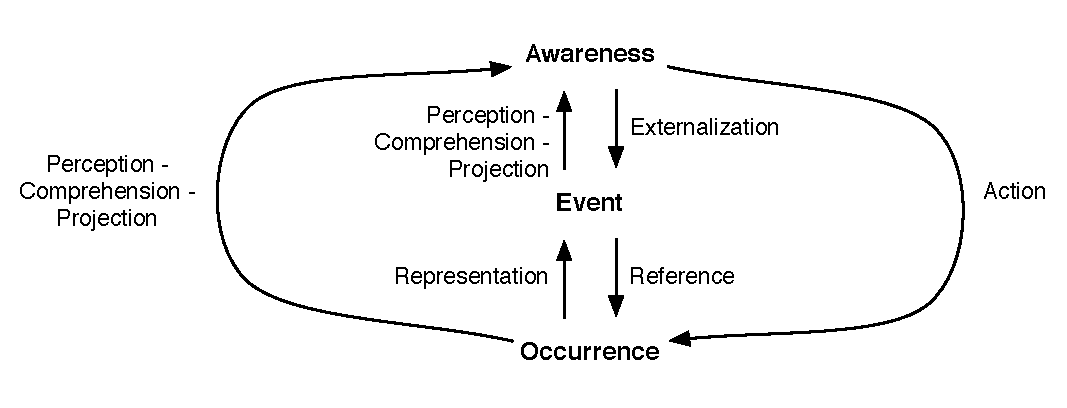
\includegraphics[width=4.5in]{occurrence_event_awareness.pdf} 
   \caption{Transformations between occurrence, event, and awareness}
   \label{fig:occurrence_event_awareness}
\end{figure}

The direct transformation between \emph{occurrence} and \emph{awareness} corresponds to the individual awareness development cycle that has been described in Section \ref{sub:awareness_as_process}. A real world \emph{occurrence} is transformed into \emph{awareness} through an actor's individual awareness processes, i.e. \emph{perception}, \emph{comprehension}, and \emph{projection}. Then, the achieved \emph{awareness} guides the actor's \emph{action} that may generate further \emph{occurrences} in the real world. 

The thing becomes more interesting when the computer support is involved and the transformations are driven by \emph{events}. One one hand is a real world \emph{occurrence} can be captured and represented as an \emph{event} by the computer system, and presented to a human actor. Instead of perceiving the \emph{occurrence} directly, the actor perceives the corresponding \emph{event} in the computer interface, and develops the \emph{awareness} upon it through the actor's individual awareness processes, i.e. \emph{perception}, \emph{comprehension}, and \emph{projection}. On the other hand is some aspect of the actor's \emph{awareness} can be externalized as a new \emph{event}, which refers to some current \emph{occurrence} or predicts future \emph{occurrence} in the real world.

The event-driven transformations can also be used to describe the different awareness propagation processes across multiple actors. The process of \emph{feedthrough} can then be described in the following steps: (1) an actor's \emph{awareness} guides his/her \emph{action} that generates a new \emph{occurrence} in the real world; (2) this new \emph{occurrence} is then captured and represented as an \emph{event} by the computer, and presented to another actor; (3) the other actor develops the \emph{awareness} upon receiving the new event. Similarly, the process of \emph{manifestation} can also be described as follow: (1) an actor's \emph{awareness} is externalized as a new \emph{event}, which refers to some current \emph{occurrence}; (2) this new \emph{event} is then presented to another actor by the computer; (3)the other actor develops the \emph{awareness} upon receiving the new event. 

Figure \ref{fig:example_awareness_traj} shows an example of how these event-driven awareness processes can be combined together to describe a complex trajectory of awareness development that involves three actors in a group. The awareness is propagated from \emph{Actor 1} to \emph{Actor 2} through the process of \emph{manifestation}, and is then propagated from \emph{Actor 2} to \emph{Actor 3} through the process of \emph{feedthrough}.

\begin{figure}[htbp] %  figure placement: here, top, bottom, or page
   \centering
   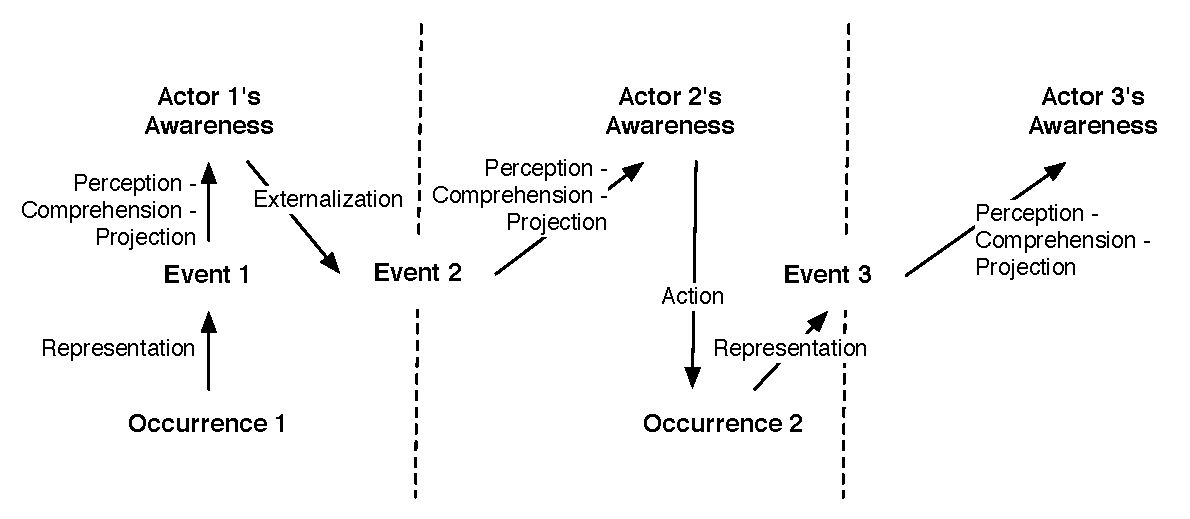
\includegraphics[width=4.5in]{example_awareness_traj.pdf} 
   \caption{An example of event-driven awareness development trajectory}
   \label{fig:example_awareness_traj}
\end{figure}
% subsubsection awareness_processes (end)
% subsection event_driven_awareness_processes (end)

\subsection{The framework} % (fold)
\label{sub:the_awareness_promotion_framework}
Built on top of the computational representation of the field of work, and the event-driven model of the awareness processes, our awareness promotion framework focuses on the interaction between these two components (Figure \ref{fig:awareness_promotion_framework}). 


\begin{figure}[htbp] %  figure placement: here, top, bottom, or page
   \centering
   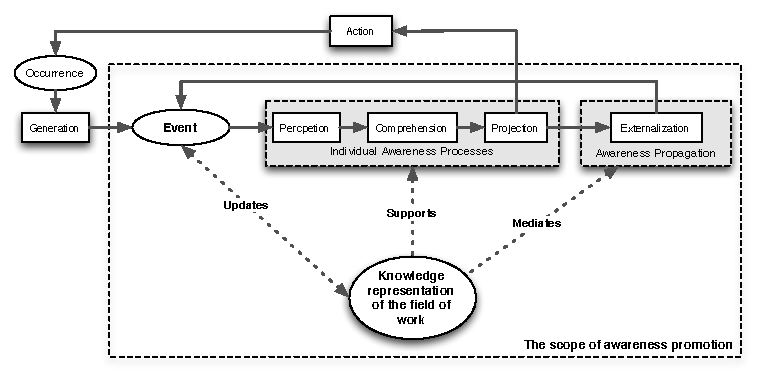
\includegraphics[width=5.5in]{awareness_promotion_framework.pdf} 
   \caption{Awareness promotion framework}
   \label{fig:awareness_promotion_framework}
\end{figure}

On one hand is how the computer constructs and develops the knowledge representation of the field of work within the event-driven processes. As we argued in Section \ref{sub:computational_representation_of_the_field_of_work}, one of the requirements for the computational representation of the field of work is that it should support dynamic adaptation so that it always reflects the current state of the changing field of work. We utilize the \emph{events} to achieve this goal. As human actors use a subset of the events to develop their individual awareness, the system processes every event to develop its knowledge representation of the whole field of work. The events can be generated by sensing the occurrences in real world, or they can be the results of human actors' externalization of their individual awareness. All of these events will be processed by the computer system to update its knowledge representation of the field of work.

On the other hand, the knowledge representation is used by the computer system to promote the awareness processes. Following the design principle of human-computer collaboration emphasizing the appropriate partition of responsibility between human actors and computer systems (Section \ref{sub:human_computer_collaboration}), the promotion role of the computer system is to strike a balance between the system's reasoning capabilities and providing visual and interactive support. With the computational knowledge about the field of work, the system can offload some of the reasoning effort from the human actors. Meanwhile, the system knowledge can also be visualized to help the human actors perform their part of the work or overwrite the computer's behaviors. 

As shown in Figure \ref{fig:awareness_promotion_framework}, we exclude the event generation process, i.e. the transformation from real world occurrences to events; and the action process, i.e. the transformation from awareness to real world occurrences, from the scope of awareness promotion in this study. It does not mean that these processes are less important or they can be separated from the rest. Rather, we believe these processes are relatively standalone processes that are out of the scope of this study, and therefore we do not claim contributions to these processes. 

The next two chapters provide details of this awareness promotion framework. Chapter \ref{cha:knowledge_reprsentation} describes the two knowledge components, i.e. the computational representation of the field of work and the specification of events, and the mechanisms for updating the knowledge representation with events. Chapter \ref{cha:promoting_event_driven_awareness} describes the promotion of individual awareness processes and awareness propagation.
% subsection the_awareness_promotion_framework (end)
% section awareness_promotion_framework (end)
% chapter our_approach_overview (end)




 

